\documentclass[compress]{beamer}
\usepackage[T1]{fontenc}

\beamertemplatenavigationsymbolsempty

%\usetheme{Madrid}

\usetheme[secheader]{Madrid}

\usepackage{mathtools,amssymb,amsthm,amsfonts,beamerthemesplit,amsmath}
\usepackage{enumerate,mathrsfs,subfig,array}

\usepackage[english]{babel}
\usepackage{csquotes}

\usepackage{graphicx}

\usepackage{color}

\usepackage{hyperref}

\usepackage{makecell}


\xdefinecolor{crimson}{RGB}{158,27,52}
\xdefinecolor{blue}{RGB}{0,124,194}
%\xdefinecolor{gray}{RGB}{0,0,0}
\xdefinecolor{gray}{RGB}{96,106,116}
\xdefinecolor{teal}{RGB}{0,177,176}
\xdefinecolor{yellow}{RGB}{235,215,34}
\xdefinecolor{darkBlue}{RGB}{12, 12, 112}

\usecolortheme[named=darkBlue]{structure}

%\usecolortheme[named=crimson]{structure}


\newtheorem{conjecture}[theorem]{Conjecture}




\setbeamertemplate{itemize items}[default]
\setbeamertemplate{enumerate items}[default]

%Shortcuts for symbol for R, C, etc
\newcommand{\N}{\mathbb{N}}
\newcommand{\Z}{\mathbb{Z}}
\newcommand{\R}{\mathbb{R}}
\newcommand{\C}{\mathbb{C}}
\newcommand{\Q}{\mathbb{Q}}
\newcommand{\F}{\mathbb{F}}
\newcommand{\E}{\mathbb{E}}
\newcommand{\T}{\mathbb{T}}
\newcommand{\K}{\mathbb{K}}
\newcommand{\X}{\mathbb{X}}
\newcommand{\Y}{\mathbb{Y}} 


\title{IOTO Goverlytic Team}

\subtitle{Coding Challenge}

\author[D. Berman, J.Glassett, D. Liu, D. Taha, A.Zheng]{Dana Berman \\Jillian Glassett \\Danyi Liu \\Diaaeldin Taha \\Aaron (Xiang) Zheng }


\date{Math$^{\text{Industry}}$, PIMS\\
August 2020}


% Delete this, if you do not want the table of contents to pop up at
% the beginning of each subsection:
\mode<presentation>{%
  %% At the begin of a section, insert a short outline
  \AtBeginSection[]{%
    \begin{frame}<beamer>%
      \frametitle{Outline}
      \tableofcontents[currentsection=show/shaded/hide]%
    \end{frame}%
  }%
  %% 
  %% Same for Subsections
  %Would produce outline again for each subsection. Could add back in.
 % \AtBeginSubsection[]{%
  %  \begin{frame}<beamer>%
  %    \frametitle{Outline}
  %    \tableofcontents[currentsection,subsectionstyle=show/shaded/hide]%
  %  \end{frame}}%
}

%As just section we are in listed at top with subsection
%instead of listing all the sections
\setbeamertemplate{headline}
{%
  \leavevmode%
  \begin{beamercolorbox}[wd=.5\paperwidth,ht=2.5ex,dp=1.125ex]{section in head/foot}%
    \hbox to .5\paperwidth{\hfil\insertsectionhead\hspace{2pt}}
  \end{beamercolorbox}%
  \begin{beamercolorbox}[wd=.5\paperwidth,ht=2.5ex,dp=1.125ex]{subsection in head/foot}%
    \hbox to .5\paperwidth{\hspace{2pt}\insertsubsectionhead\hfil}
  \end{beamercolorbox}%
}
%Gets ride of navigation symbols
\setbeamertemplate{navigation symbols}{} 

% Let's get started
\begin{document}

\begin{frame}
  \titlepage
\end{frame}


%%%%Only need to introduce team members, don't need to show profiles

%\section*{Profiles}

%\frame{\frametitle{Profiles}

%%Each name is a link to be clicked on; opens up m2pi.ca profile
%\begin{itemize}
%    \item \href{https://m2pi.ca/authors/dana996/}{Dana Berman}
%    \item \href{https://m2pi.ca/authors/jlglassett/}{Jillian Glassett}
%    \item \href{https://m2pi.ca/authors/danyi-liu/}{Danyi Liu}
%    \item \href{https://m2pi.ca/authors/d-ta/}{Diaaeldin Taha}
%    \item \href{https://m2pi.ca/authors/umaaron/}{Aaron (Xiang) Zheng}
%   
%\end{itemize}


%}

%\begin{frame}{Outline of Coding Challenge}
%  \tableofcontents

%\end{frame}

% Section and subsections will appear in the presentation overview
% and table of contents.

\section{Overview of the Data}


\begin{frame}
The GC Service Inventory dataset
\vfill
\begin{itemize}
	\item Bird’s-eye-view of services provided by some departments of the Government of Canada (GC)
%	\item is available online on the GC Open Government website

\vfill
	\item Reports over three fiscal years:
	\begin{itemize}
	    \item 2016-2017, 2017-2018, and 2018-2019
	\end{itemize}
\vfill	

	\item Includes:
	\begin{itemize}
        \item Service description (name, department, etc.)
        \item Number of web visits, applications, phone calls
        \item Service fee, SIN used, 
    \end{itemize}
\vfill	
\end{itemize}

%We focus on categorical and numerical data in order to present important insights and correlations.
\end{frame}



\begin{frame}{First Impressions}
%Dia and Aaron's line plots
%Mean, range, std, etc.??
%Notable missing data---> excluded last fiscal year for this reason


%Dia's graph of total apps

\begin{itemize}
    \item First two years on 11 departments
    \item Third year expanded to 67 departments
\end{itemize}

%The Open Government initiative expanded data collection from \textbf{11} departments in the years 2016-2017, 2017-2018 to \textbf{67} departments in the year 2018-2019. 

\begin{figure}
\centering
\begin{minipage}{0.5\textwidth}
  \centering
  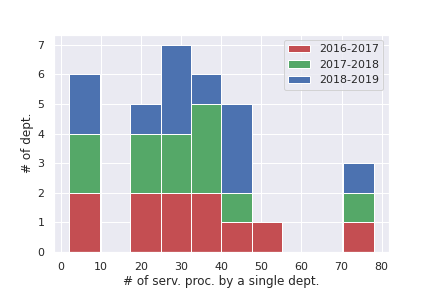
\includegraphics[width=\linewidth]{number_services_hist_1.png}
\end{minipage}%
\begin{minipage}{.5\textwidth}
  \centering
  \includegraphics[width=\linewidth]{number_services_hist_2.png}
\end{minipage}
\caption{\small{Num. of services provided per department for (left) the common 11 departments over three fiscal years, and (right) all departments during the third year.}}
\end{figure}

\hfill\tiny{Plots by: Dia Taha}


%PLus Aaron's graph seperating by applictions

%Noting the change in webservice for only employment
%and drop of online application for two branches
%-> 2018-2019 from closer look had more missing info
%-> decided to look closer at first tow fiscal years
    
\end{frame}


\section{Main Observations}

%\subsection{Results (1)}
\begin{frame}{Number of applications per Fiscal Year}
%Main plot 2 goes here
\begin{figure}[htp]
    \centering
    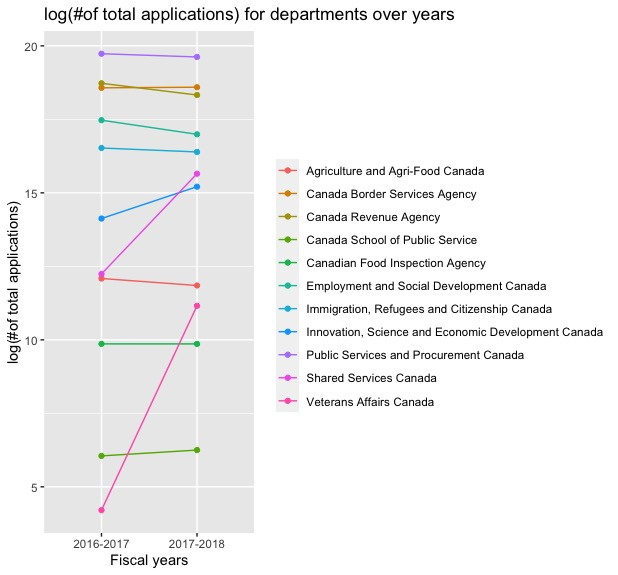
\includegraphics[width=7.5cm]{2.jpeg}
    %\caption{log(\#of total applications) for departments over years}
\end{figure}

\hfill\tiny{Plot by: Danyi Liu}
\end{frame}


\begin{frame}{Web Visits v.s. Total Applications }
   % As one would expect, there is some correlation between the number of applications and the number of web visits. However, as will become clear in later slides, there are many factors will influence the number of applications.
   
   Some correlation between number of applications and number of web visits.
   \vfill
    %Main plot 1 goes here
    \begin{figure}
        \centering
        \includegraphics[width = \textwidth]{web_app_scatter.png}
        \label{fig:my_label}
    \end{figure}
    %Log scatter plot of apps (Dana's graph) comparing web visits and number of applications
    \vfill
\hfill\tiny{Plot by: Dana Berman}
\end{frame}




%\subsection{Result 2}
\begin{frame}{Service Fees Affecting Applications}
\begin{figure}[htp]
    \centering
    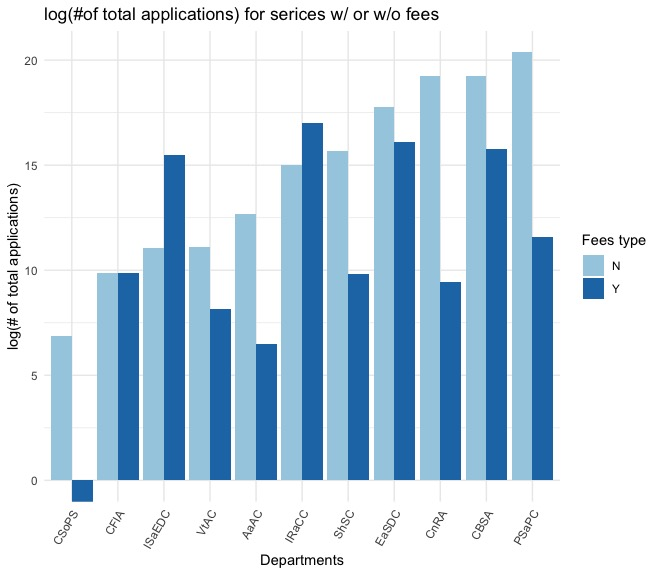
\includegraphics[width=8cm]{3.jpeg}
\end{figure}
\hfill\tiny{Plot by: Danyi Liu}
\end{frame}


\begin{frame}{Electronic Enabled Services}
\begin{figure}[htp]
    \centering
    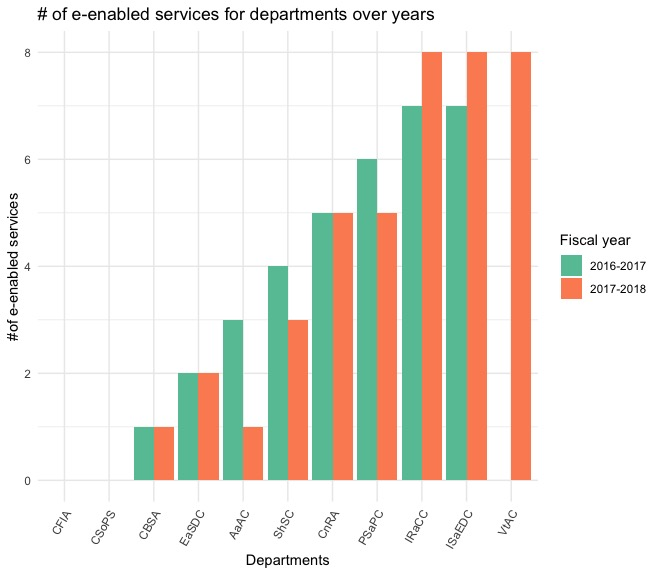
\includegraphics[width=8cm]{4.jpeg}
\end{figure}
\hfill\tiny{Plot by: Danyi Liu}
\end{frame}


% Placing a * after \section means it will not show in the
% outline or table of contents.
%\section*{Summary}

\begin{frame}{Summary}
\begin{itemize}
    \item Connection between web visits and applications
    \vfill
    \item Some connections between service fees and applications
    \vfill
    \item Differences between departments on electronic services.
  
    \vfill
    \item Other connections may exist, but missing data
    \vfill
\end{itemize}
\end{frame}

% All of the following is optional and typically not needed. 
\appendix
\section<presentation>*{\appendixname}
\subsection<presentation>*{Sources}

\begin{frame}[allowframebreaks]
  \frametitle<presentation>{Sources}
    
  \begin{thebibliography}{10}
    
  %\beamertemplatebookbibitems
  % Start with overview books.
  
  \bibitem{GC_dataset}
  Government of Canada. \emph{GC Service Inventory Dataset}. June 30, 2020. Distributed by GC Open Government.
  \newblock \url{https://open.canada.ca/data/en/dataset/3ac0d080-6149-499a-8b06-7ce5f00ec56c}
  \newblock Accessed: 2020-08-13
  
  %Add git-hub repo once public?
  
  
  \end{thebibliography}
\end{frame}

\begin{frame}\frametitle{Thank you}
\begin{center}
Thank you for your time!\\
\end{center}

\end{frame}

\end{document}


